\chapter{Tests des Robotersystems}
\label{cha:Tests}
\section{Tests im gesicherten Rahmen}

\section{Realtests}

\subsection*{Manuelle Steuerung}

Zum Testen der Fahrfähigkeit, des Greifarms und der Positionsverfolgung wurde unter dem Einstellungsmenü der CLEEN-R App der Menüpunkt "manuelle Kontrolle" hinzugefügt. Über ihn wird die in Bild \ref{fig:manualControl} Activity gestartet, die dem Benutzer oder Tester die Kontrolle über die Bewegungen des Roboters gibt.

\begin{figure}[h]
\centering
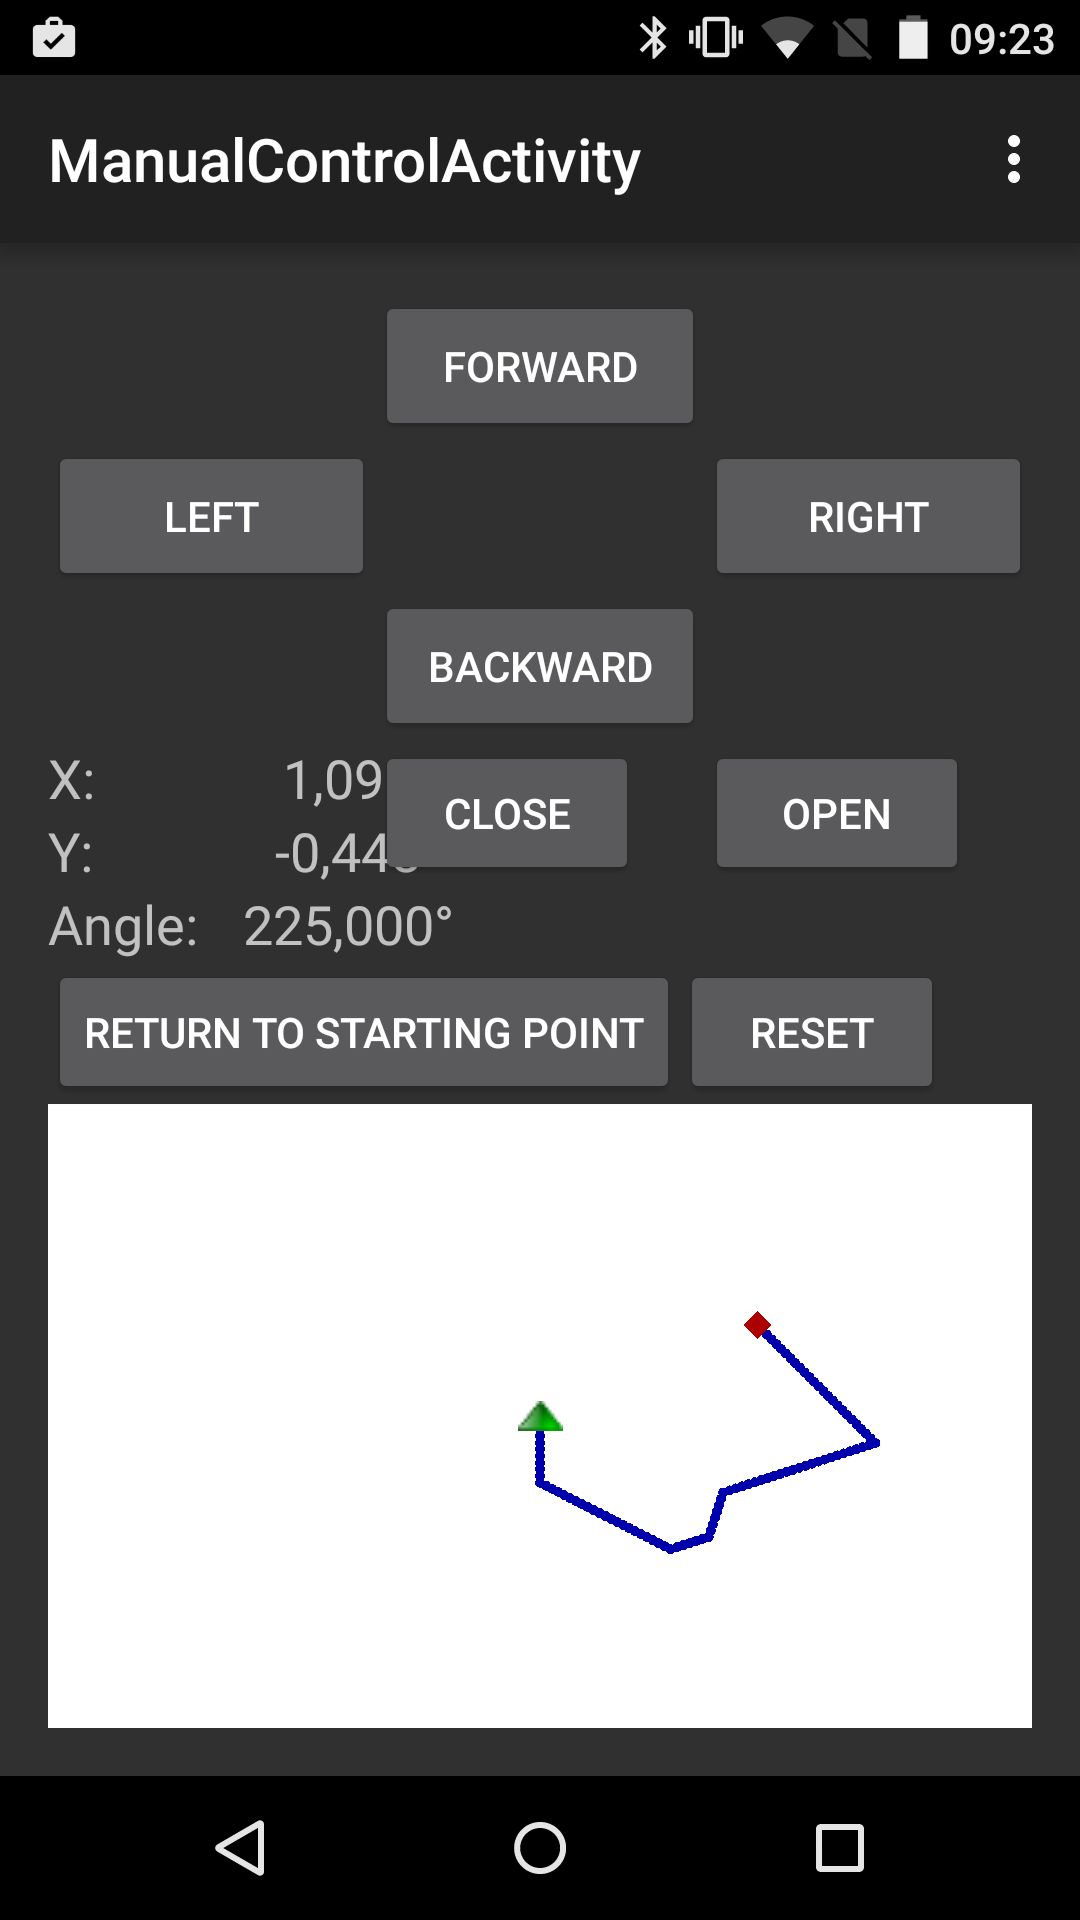
\includegraphics[width=0.4\textwidth]{Bilder/Tests/manualControl}
\caption{Manuelle Steuerung des Roboters}
\label{fig:manualControl}
\end{figure}

Das Smartphone wird für die direkte Kontrolle vom Roboter in die Hand genommen, die Übertragung der Befehle erfolgt wie im Normalbetrieb via Bluetooth.

Über Buttons kann sowohl vor- und rückwärts gefahren, als auch im und gegen den Uhrzeigersinn rotiert werden. Des Weiteren lässt sich der Greifarm beliebig weit öffnen und schließen. Die aktuelle Position und der Winkel im Vergleich zum Start wird in Koordinatenform angezeigt und während der Bewegungen aktualisiert.

Im unteren Teil des Bildschirms befindet sich eine graphische Repräsentation des Roboters und des bereits zurückgelegten Weges durch das Zimmer, der Startpunkt wird ebenfalls markiert.

Nach dem manuellen Anfahren und Aufnehmen eines Objekts kann über einen Knopf der Roboter wie in Kapitel \ref{sec:Rückkehr} vollautomatisch zum Startpunkt zurückgefahren werden.
